\chapter{Lab 7: UART} \label{day7}

In this lab we learn how to transmit data between a PC and the \gls{fpga} board with an ``UART''-transmitter and how to ensure correct transmission with oversampling.

\section{Direct loop-back}

This simple program connects the receiver port (RX) to the transmitter port (TX) and a second pin that we connected to the logic analyzer. After opening the terminal program with ``picocom -b 115200 /dev/ttyUSB1'' we could send data to the board and analyze the output of the board with the logic analyzer software.

\lstinputlisting[language=VHDL]{./L7/E1/src/project_7_1.vhd}

% kommentierten Code vielleicht noch entfernen

\begin{figure}[h]
	\centering
	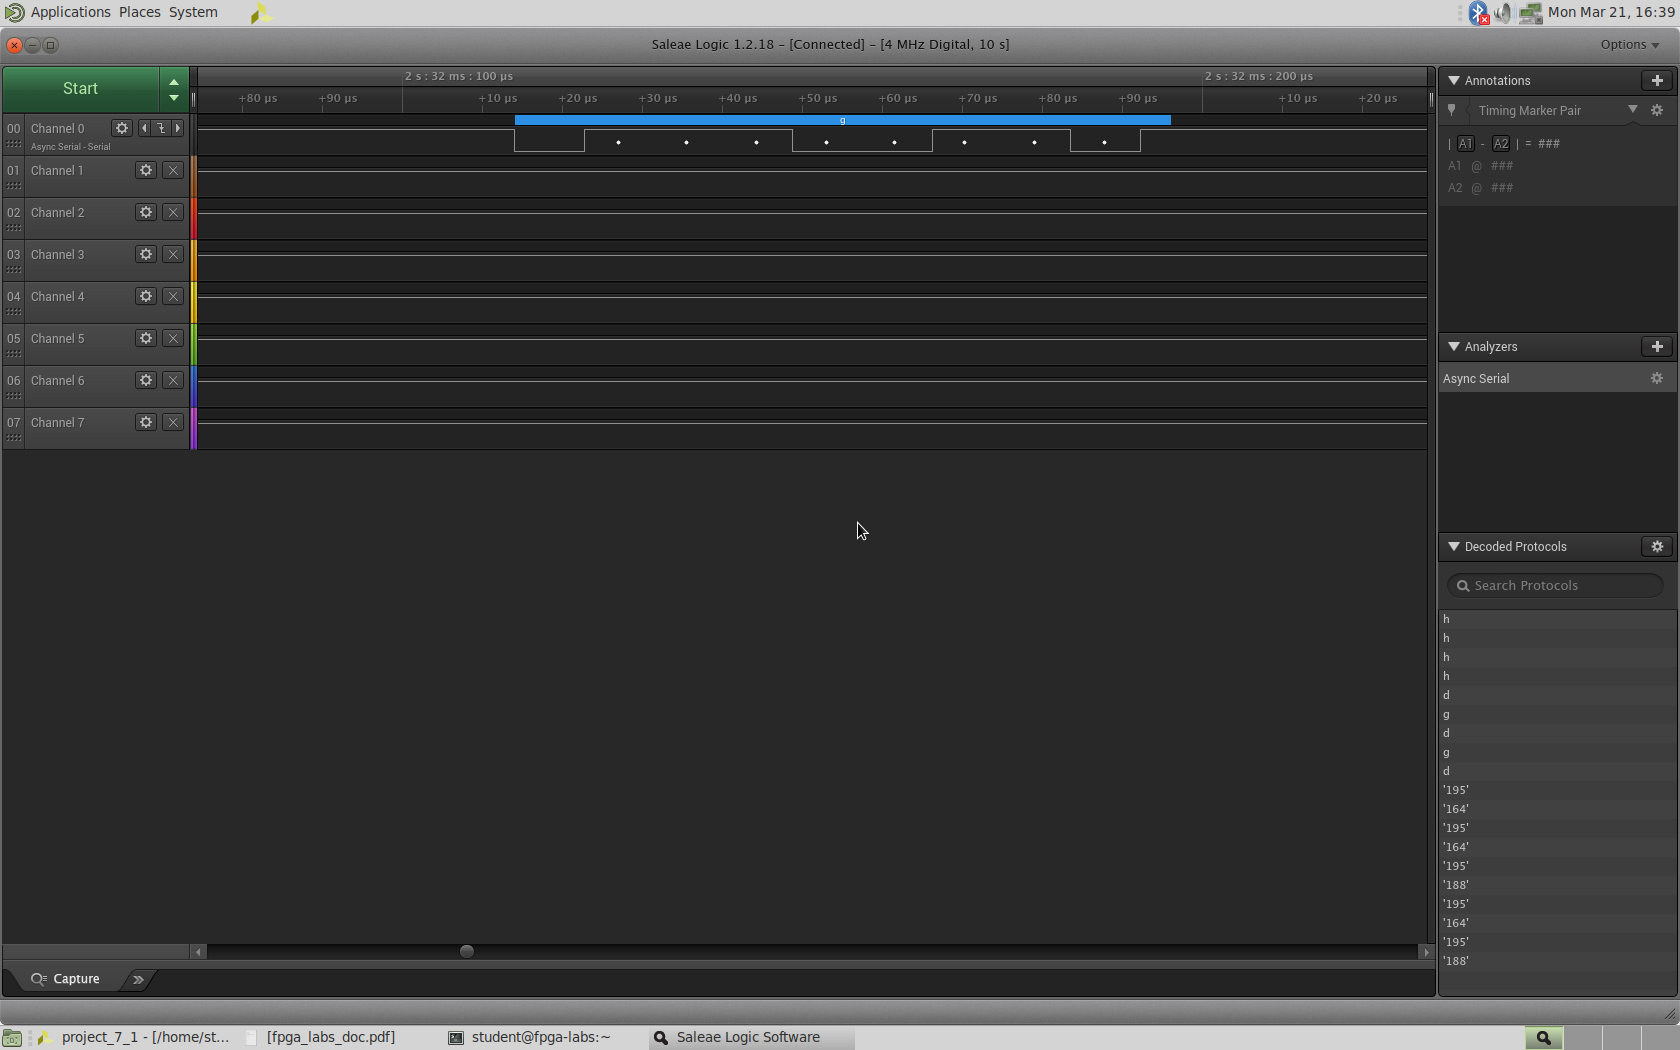
\includegraphics[width=\linewidth]{./L7/E1/example_transmission.png}
	\caption{The logic analyzer software. Here, the input of the terminal program can be seen as transmitted bits.} 
	\label{fig: logic analyzer software e_7_1}
\end{figure}

\section{UART sender}

This UART sender send data from the \gls{fpga} to the computer. Here, switches on the \gls{fpga} board are used as the input to be transmitted and a button as enter. Therefore we reused the debouncer for the button from the previous exercise 3.1 as well as a timer module with an output frequency of 115200\,Hz. The actual frequency is 11428\,Hz (see fig. \ref{fig: transmitted information e_7_2}) which is no problem for the receiver.

\begin{figure}[!htb]
	\centering
	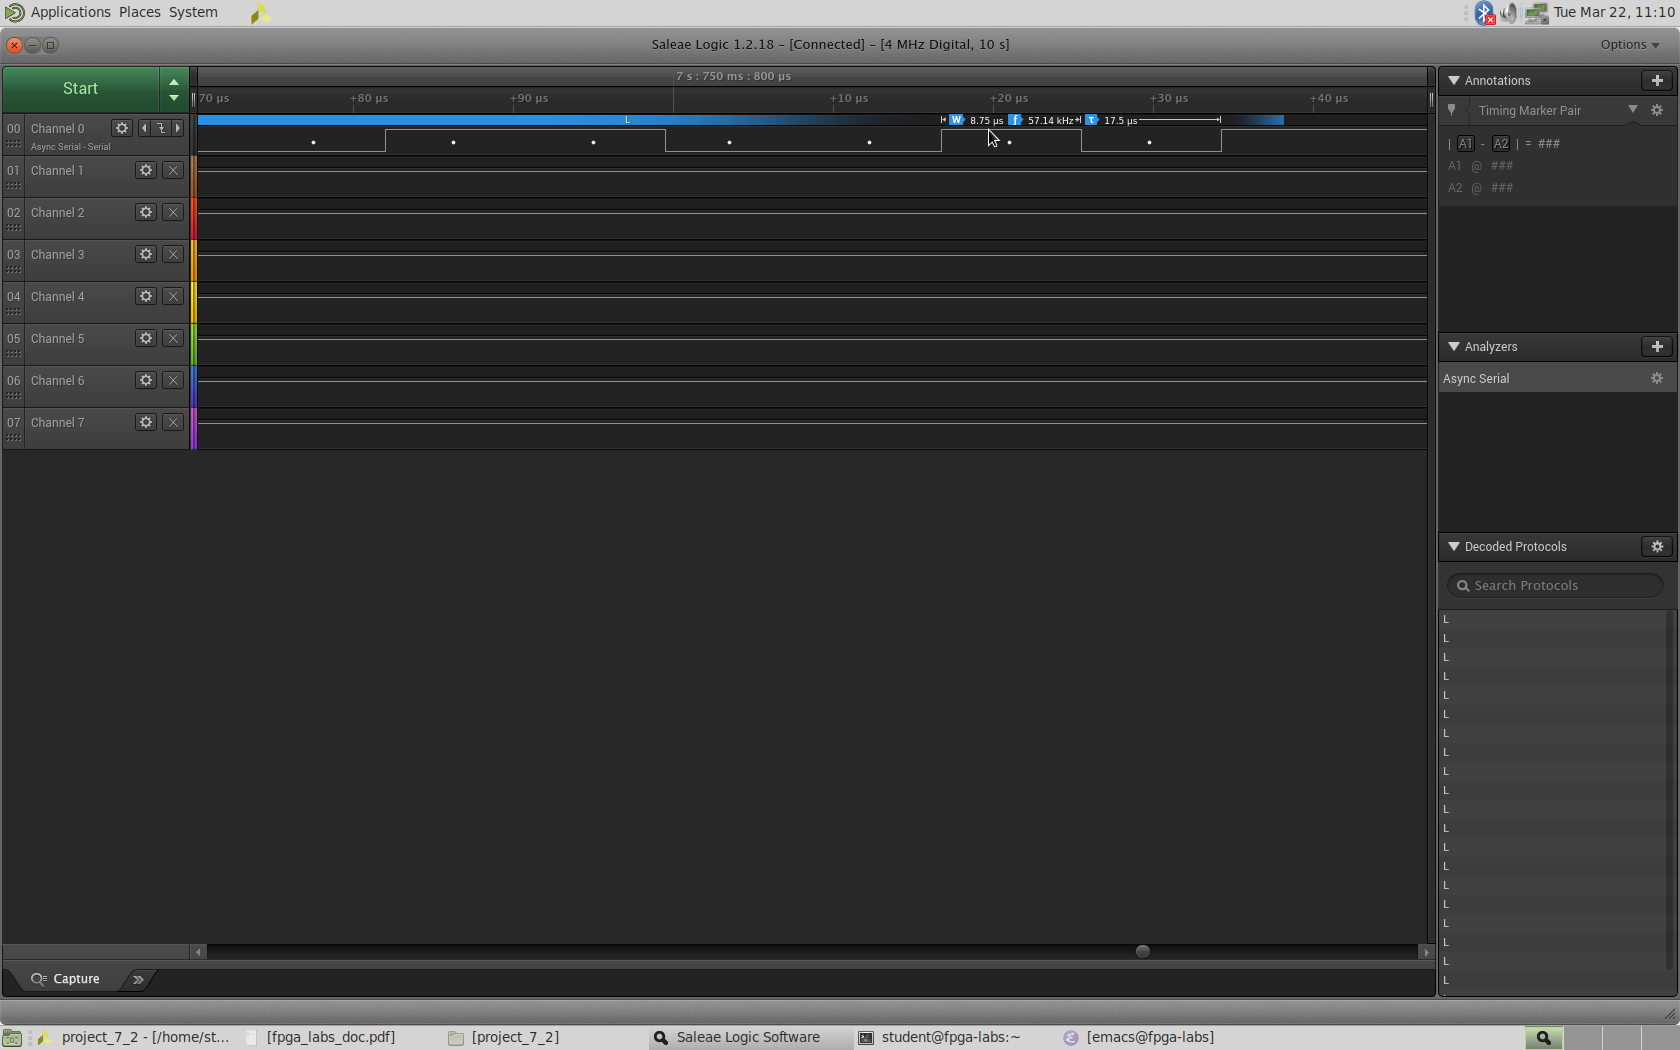
\includegraphics[width=\linewidth]{./L7/E2/freq.png}
	\caption{The transmitted information ``L'' is read out with the logic analyzer. } 
	\label{fig: transmitted information e_7_2}
\end{figure}

\lstinputlisting[language=VHDL]{./L7/E2/src/project_7_2.vhd}

\lstinputlisting[language=VHDL]{./L7/E2/src/project_7_2_1.vhd}

\section{Simple UART receiver}

Here, we receive data from the computer over the receiver port (RX) on the \gls{fpga} and display the number of framing errors on the display. That has been realized by checking if the ``STOP'' bit after transmission is 1. If the received ``STOP'' bit is 0 the error counter increases. The ``VALID'' and ``ERROR'' bits are displayed with the LEDs of the board. 

\lstinputlisting[language=VHDL]{./L7/E3/src/project_7_3.vhd}

\lstinputlisting[language=VHDL]{./L7/E3/src/project_7_3_1.vhd}

\lstinputlisting[language=VHDL]{./L7/E3/src/project_7_3_tb.vhd}

Sending 100 characters to the board we received no errors. Although when pressing a button of the computer keyboard continuously we received some errors.

% Wie sollten wir das mit dem Error Zähler beschreiben, der hat ja nicht hochgezählt¿

\section{Oversampling UART receiver}

To eliminate remaining transmission errors oversampling can be used to facilitate the receiver. By waiting for a short period of time after receiving the ``START'' bit the receiver can save the transmitted information without any clock discrepancies.

\lstinputlisting[language=VHDL]{./L7/E3/src/project_7_3.vhd}

\lstinputlisting[language=VHDL]{./L7/E3/src/project_7_3_1.vhd}
